\question
\begin{parts}
	\part You release a proton from rest in the presence of an unknown force field. Seconds later, you measure the velocity of the proton to be 450 m/s. Which force(s) may have contributed to this acceleration? (Circle all that apply, and justify your answer).
	\begin{enumerate}
		\item Gravitational Field
		\item Magnetic Field
		\item Electric Field
		\item Hydrostatic Field
	\end{enumerate}

	\part Several positive charges are placed at the center of a solid insulating sphere
	
	\begin{figure}[ht!]
		\centering
		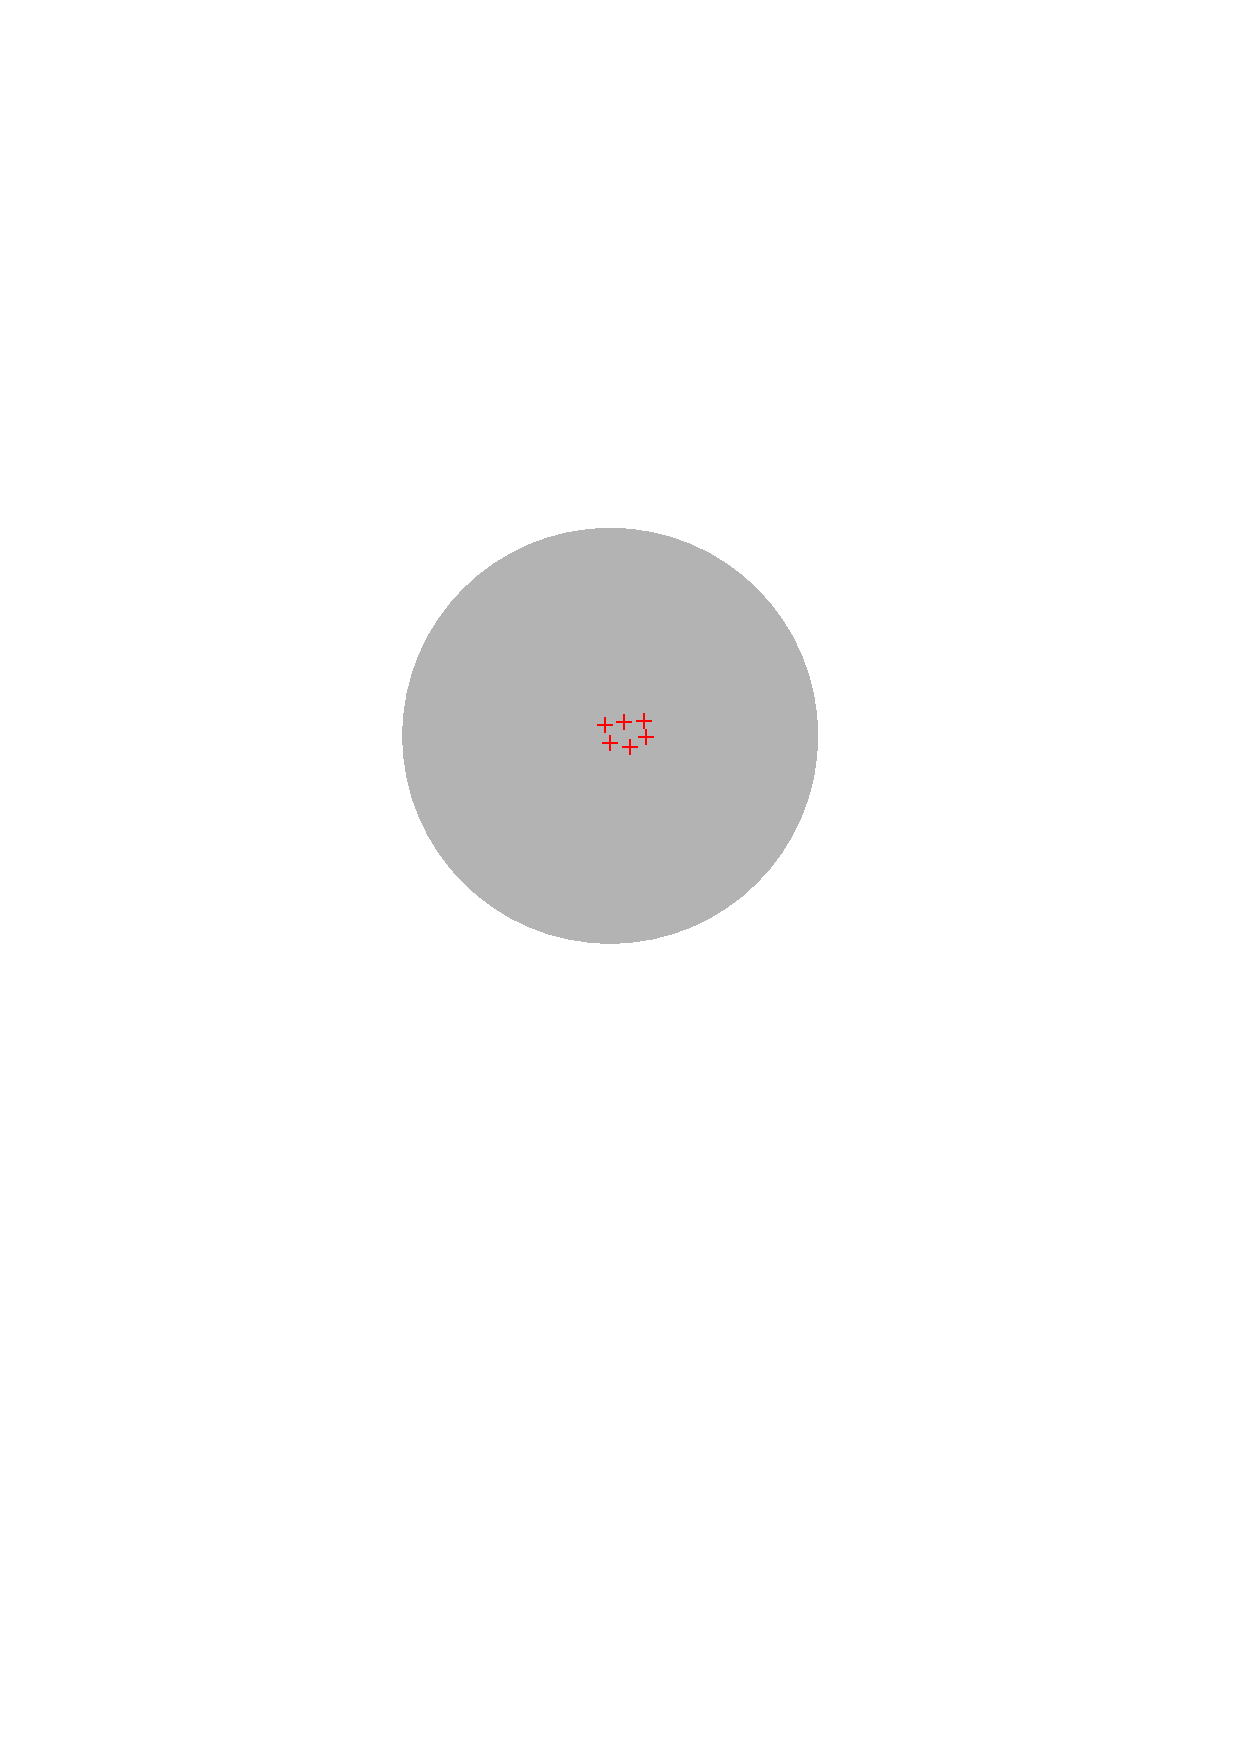
\includegraphics[width=5cm]{sphere_dist}
	\end{figure}

	\begin{subparts}
	\subpart Sketch the approximate charge distribution a few seconds later (long after any equilibrium has been reached)
	
	\subpart The exact process is repeated, this time for a solid conducting sphere. Once again, sketch the approximate charge distribution several seconds later.
	\end{subparts}

	\part For each of the four electric field patterns shown below, sketch a possible charge distribution responsible for creating that field. If the field is not possible, say so and explain why.\\
	\begin{tabular}{cc}
		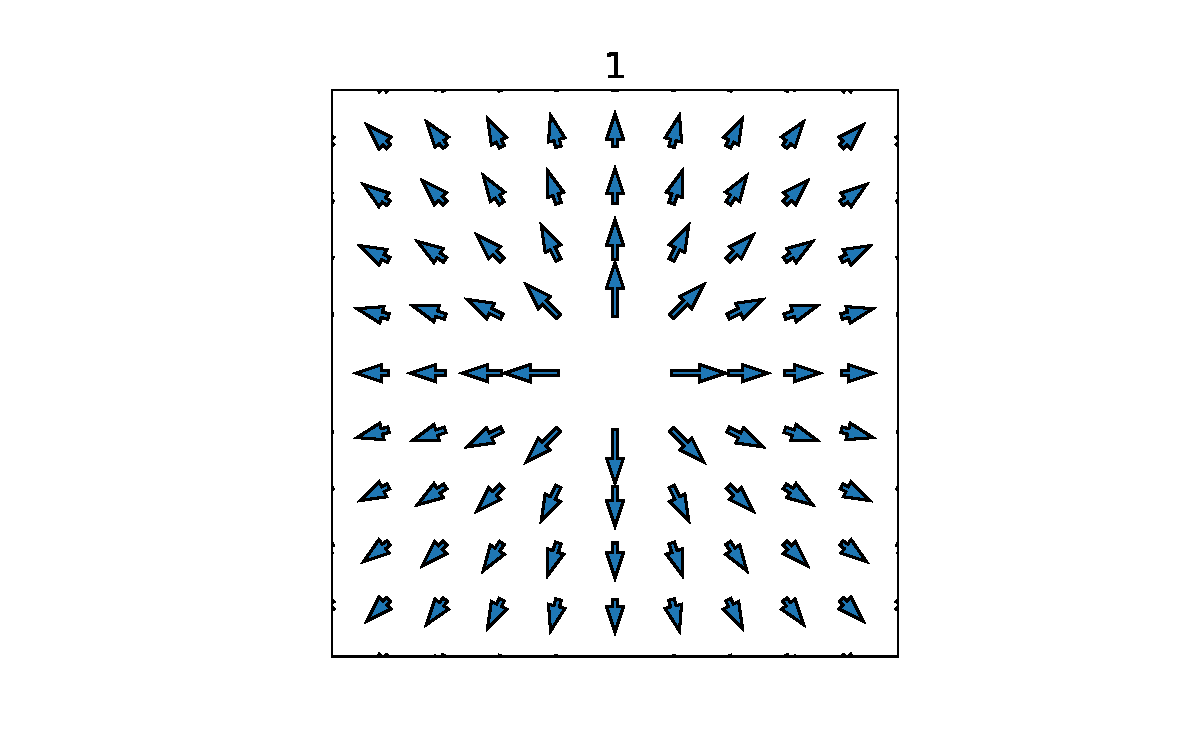
\includegraphics[width=8cm]{inverse_square_field.pdf} & 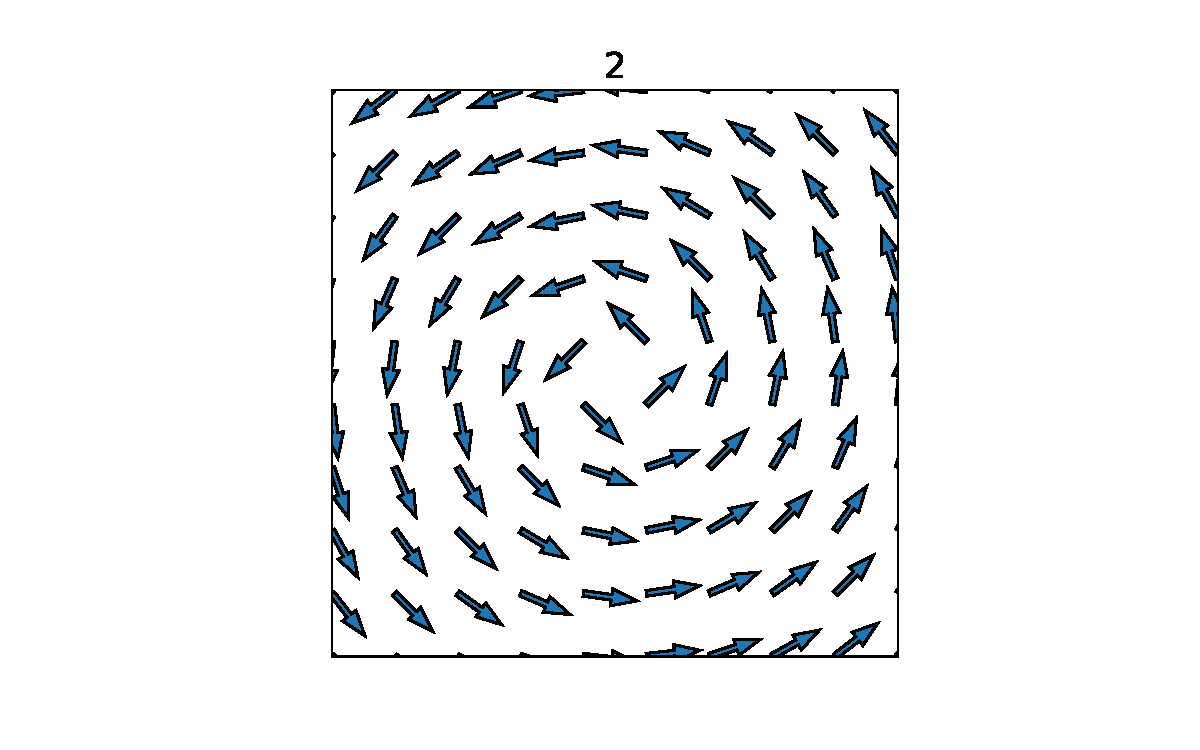
\includegraphics[width=8cm]{invalid_field.pdf}\\
		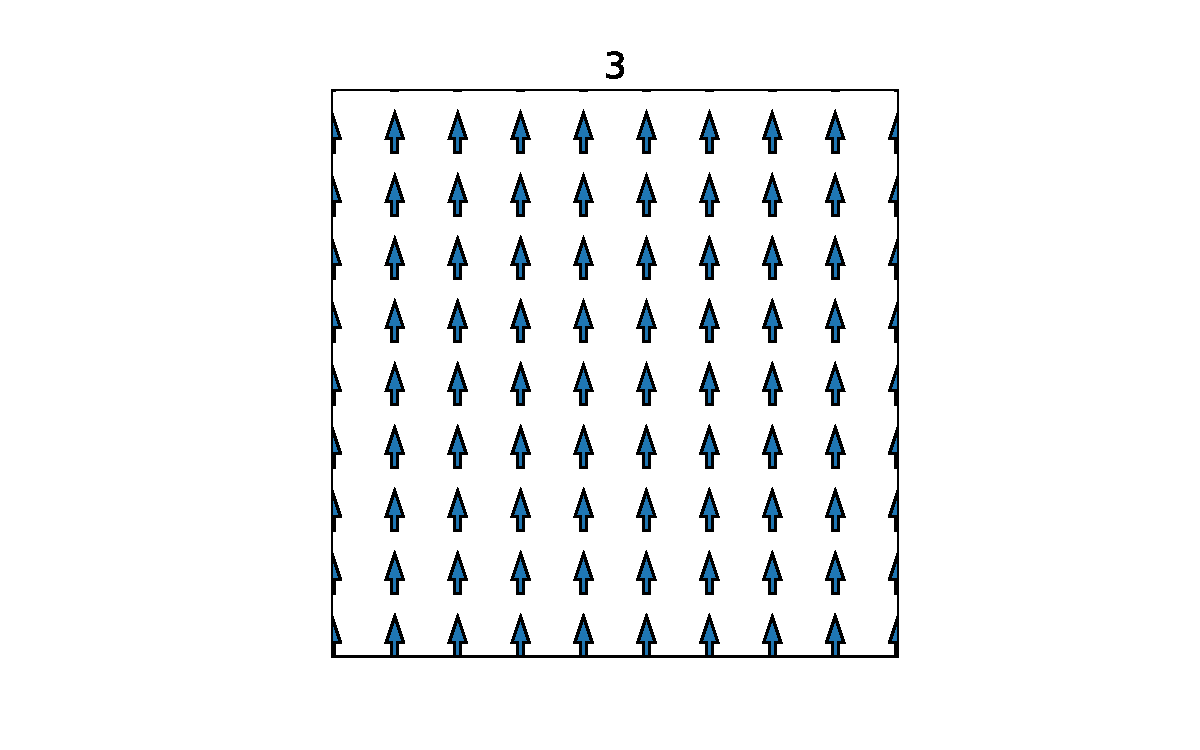
\includegraphics[width=8cm]{capacitor_field.pdf} & 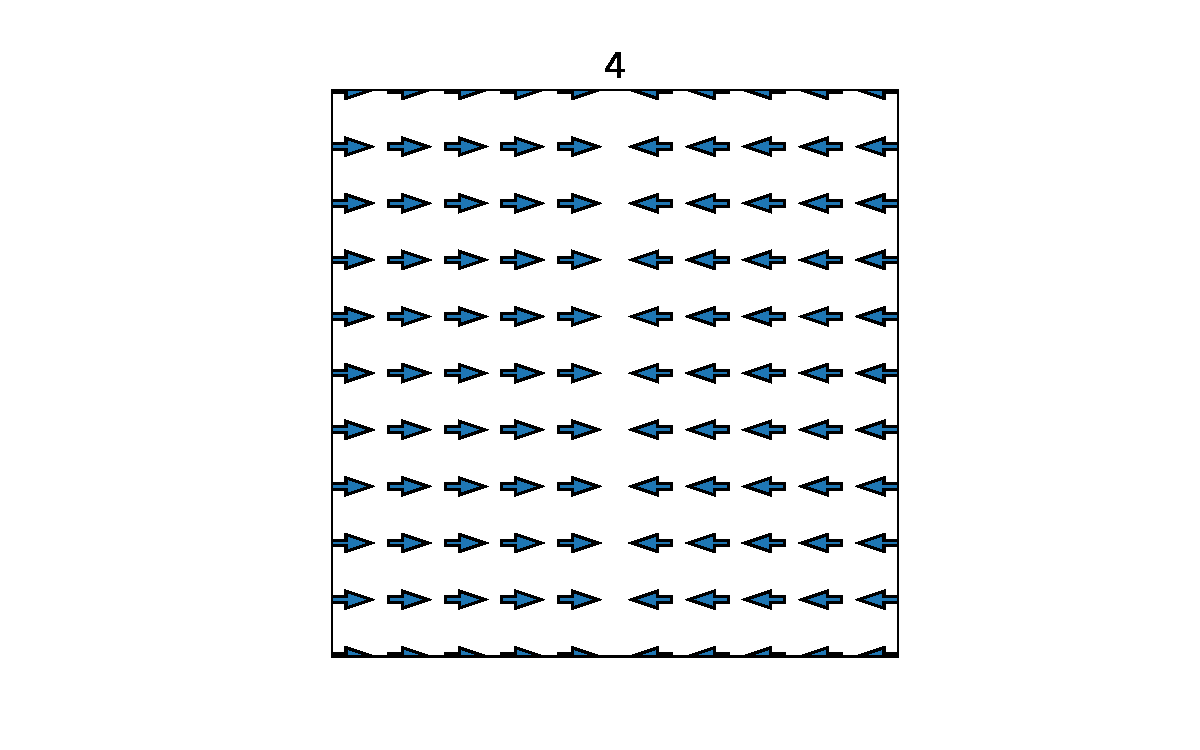
\includegraphics[width=8cm]{neg_sheet_field.pdf}
	\end{tabular}
\end{parts}